\documentclass[ignorenonframetext,]{beamer}
\setbeamertemplate{caption}[numbered]
\setbeamertemplate{caption label separator}{: }
\setbeamercolor{caption name}{fg=normal text.fg}
\beamertemplatenavigationsymbolsempty
\usepackage{lmodern}
\usepackage{amssymb,amsmath}
\usepackage{ifxetex,ifluatex}
\usepackage{fixltx2e} % provides \textsubscript
\ifnum 0\ifxetex 1\fi\ifluatex 1\fi=0 % if pdftex
  \usepackage[T1]{fontenc}
  \usepackage[utf8]{inputenc}
\else % if luatex or xelatex
  \ifxetex
    \usepackage{mathspec}
  \else
    \usepackage{fontspec}
  \fi
  \defaultfontfeatures{Ligatures=TeX,Scale=MatchLowercase}
\fi
\usefonttheme{structurebold}
% use upquote if available, for straight quotes in verbatim environments
\IfFileExists{upquote.sty}{\usepackage{upquote}}{}
% use microtype if available
\IfFileExists{microtype.sty}{%
\usepackage{microtype}
\UseMicrotypeSet[protrusion]{basicmath} % disable protrusion for tt fonts
}{}
\newif\ifbibliography
\usepackage{color}
\usepackage{fancyvrb}
\newcommand{\VerbBar}{|}
\newcommand{\VERB}{\Verb[commandchars=\\\{\}]}
\DefineVerbatimEnvironment{Highlighting}{Verbatim}{commandchars=\\\{\}}
% Add ',fontsize=\small' for more characters per line
\usepackage{framed}
\definecolor{shadecolor}{RGB}{248,248,248}
\newenvironment{Shaded}{\begin{snugshade}}{\end{snugshade}}
\newcommand{\KeywordTok}[1]{\textcolor[rgb]{0.13,0.29,0.53}{\textbf{{#1}}}}
\newcommand{\DataTypeTok}[1]{\textcolor[rgb]{0.13,0.29,0.53}{{#1}}}
\newcommand{\DecValTok}[1]{\textcolor[rgb]{0.00,0.00,0.81}{{#1}}}
\newcommand{\BaseNTok}[1]{\textcolor[rgb]{0.00,0.00,0.81}{{#1}}}
\newcommand{\FloatTok}[1]{\textcolor[rgb]{0.00,0.00,0.81}{{#1}}}
\newcommand{\ConstantTok}[1]{\textcolor[rgb]{0.00,0.00,0.00}{{#1}}}
\newcommand{\CharTok}[1]{\textcolor[rgb]{0.31,0.60,0.02}{{#1}}}
\newcommand{\SpecialCharTok}[1]{\textcolor[rgb]{0.00,0.00,0.00}{{#1}}}
\newcommand{\StringTok}[1]{\textcolor[rgb]{0.31,0.60,0.02}{{#1}}}
\newcommand{\VerbatimStringTok}[1]{\textcolor[rgb]{0.31,0.60,0.02}{{#1}}}
\newcommand{\SpecialStringTok}[1]{\textcolor[rgb]{0.31,0.60,0.02}{{#1}}}
\newcommand{\ImportTok}[1]{{#1}}
\newcommand{\CommentTok}[1]{\textcolor[rgb]{0.56,0.35,0.01}{\textit{{#1}}}}
\newcommand{\DocumentationTok}[1]{\textcolor[rgb]{0.56,0.35,0.01}{\textbf{\textit{{#1}}}}}
\newcommand{\AnnotationTok}[1]{\textcolor[rgb]{0.56,0.35,0.01}{\textbf{\textit{{#1}}}}}
\newcommand{\CommentVarTok}[1]{\textcolor[rgb]{0.56,0.35,0.01}{\textbf{\textit{{#1}}}}}
\newcommand{\OtherTok}[1]{\textcolor[rgb]{0.56,0.35,0.01}{{#1}}}
\newcommand{\FunctionTok}[1]{\textcolor[rgb]{0.00,0.00,0.00}{{#1}}}
\newcommand{\VariableTok}[1]{\textcolor[rgb]{0.00,0.00,0.00}{{#1}}}
\newcommand{\ControlFlowTok}[1]{\textcolor[rgb]{0.13,0.29,0.53}{\textbf{{#1}}}}
\newcommand{\OperatorTok}[1]{\textcolor[rgb]{0.81,0.36,0.00}{\textbf{{#1}}}}
\newcommand{\BuiltInTok}[1]{{#1}}
\newcommand{\ExtensionTok}[1]{{#1}}
\newcommand{\PreprocessorTok}[1]{\textcolor[rgb]{0.56,0.35,0.01}{\textit{{#1}}}}
\newcommand{\AttributeTok}[1]{\textcolor[rgb]{0.77,0.63,0.00}{{#1}}}
\newcommand{\RegionMarkerTok}[1]{{#1}}
\newcommand{\InformationTok}[1]{\textcolor[rgb]{0.56,0.35,0.01}{\textbf{\textit{{#1}}}}}
\newcommand{\WarningTok}[1]{\textcolor[rgb]{0.56,0.35,0.01}{\textbf{\textit{{#1}}}}}
\newcommand{\AlertTok}[1]{\textcolor[rgb]{0.94,0.16,0.16}{{#1}}}
\newcommand{\ErrorTok}[1]{\textcolor[rgb]{0.64,0.00,0.00}{\textbf{{#1}}}}
\newcommand{\NormalTok}[1]{{#1}}
\usepackage{graphicx,grffile}
\makeatletter
\def\maxwidth{\ifdim\Gin@nat@width>\linewidth\linewidth\else\Gin@nat@width\fi}
\def\maxheight{\ifdim\Gin@nat@height>\textheight0.8\textheight\else\Gin@nat@height\fi}
\makeatother
% Scale images if necessary, so that they will not overflow the page
% margins by default, and it is still possible to overwrite the defaults
% using explicit options in \includegraphics[width, height, ...]{}
\setkeys{Gin}{width=\maxwidth,height=\maxheight,keepaspectratio}

% Prevent slide breaks in the middle of a paragraph:
\widowpenalties 1 10000
\raggedbottom

\AtBeginPart{
  \let\insertpartnumber\relax
  \let\partname\relax
  \frame{\partpage}
}
\AtBeginSection{
  \ifbibliography
  \else
    \let\insertsectionnumber\relax
    \let\sectionname\relax
    \frame{\sectionpage}
  \fi
}
\AtBeginSubsection{
  \let\insertsubsectionnumber\relax
  \let\subsectionname\relax
  \frame{\subsectionpage}
}

\setlength{\emergencystretch}{3em}  % prevent overfull lines
\providecommand{\tightlist}{%
  \setlength{\itemsep}{0pt}\setlength{\parskip}{0pt}}
\setcounter{secnumdepth}{0}
\definecolor{links}{HTML}{800080}
\hypersetup{colorlinks,linkcolor=,urlcolor=links}

\title{Web Data Collection with R}
\subtitle{HTTP}
\author{Peter Meißner / 2016-02-29 -- 2016-03-04 / ECPR WSMT}
\date{}

\begin{document}
\frame{\titlepage}

\begin{frame}
\tableofcontents[hideallsubsections]
\end{frame}

\section{Teaser}\label{teaser}

\begin{frame}{URL example}

\url{https://en.wikipedia.org/wiki/Lion}
\url{http://r-datacollection.com}

400 page not found 503 intenal server error 200 ok

\end{frame}

\begin{frame}[fragile]{things returned by httr functions}

\begin{Shaded}
\begin{Highlighting}[]
\KeywordTok{library}\NormalTok{(httr)}

\NormalTok{res <-}\StringTok{ }\KeywordTok{GET}\NormalTok{(}\StringTok{"example.com"}\NormalTok{)}

\KeywordTok{names}\NormalTok{(res)}
\end{Highlighting}
\end{Shaded}

\begin{verbatim}
##  [1] "url"         "status_code" "headers"     "all_headers" "cookies"    
##  [6] "content"     "date"        "times"       "request"     "handle"
\end{verbatim}

\begin{Shaded}
\begin{Highlighting}[]
\NormalTok{res$url}
\end{Highlighting}
\end{Shaded}

\begin{verbatim}
## [1] "HTTP://example.com/"
\end{verbatim}

\begin{Shaded}
\begin{Highlighting}[]
\NormalTok{res$status_code}
\end{Highlighting}
\end{Shaded}

\begin{verbatim}
## [1] 200
\end{verbatim}

\end{frame}

\begin{frame}{client server communication}

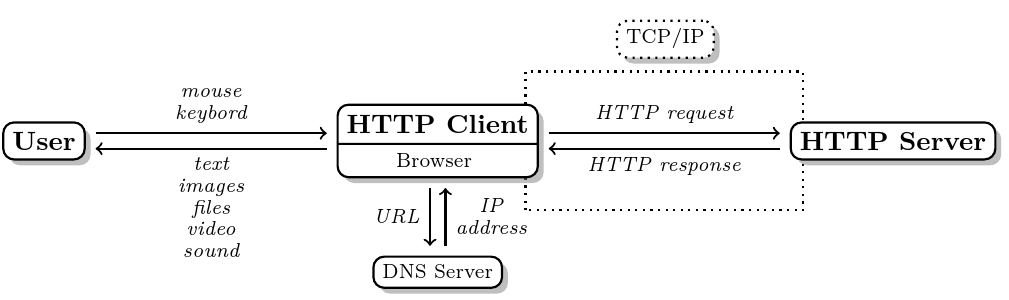
\includegraphics{fig/clientserver.png}

\end{frame}

\begin{frame}{HTTP requests}

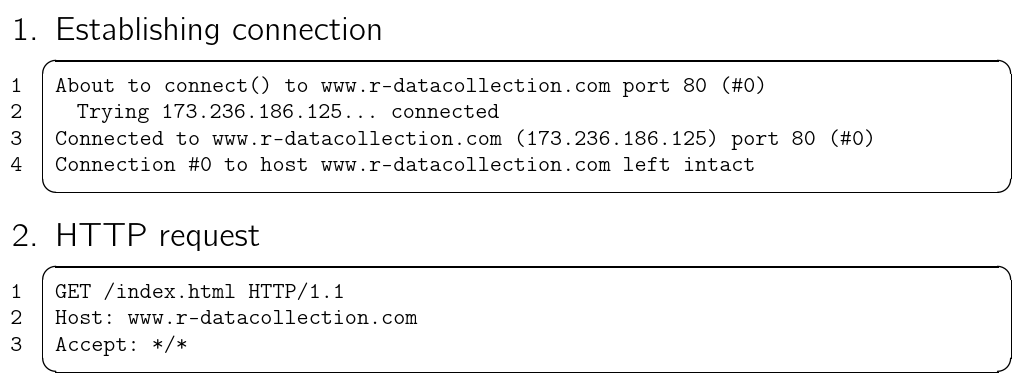
\includegraphics{fig/request.png}

\end{frame}

\begin{frame}{HTTP responses}

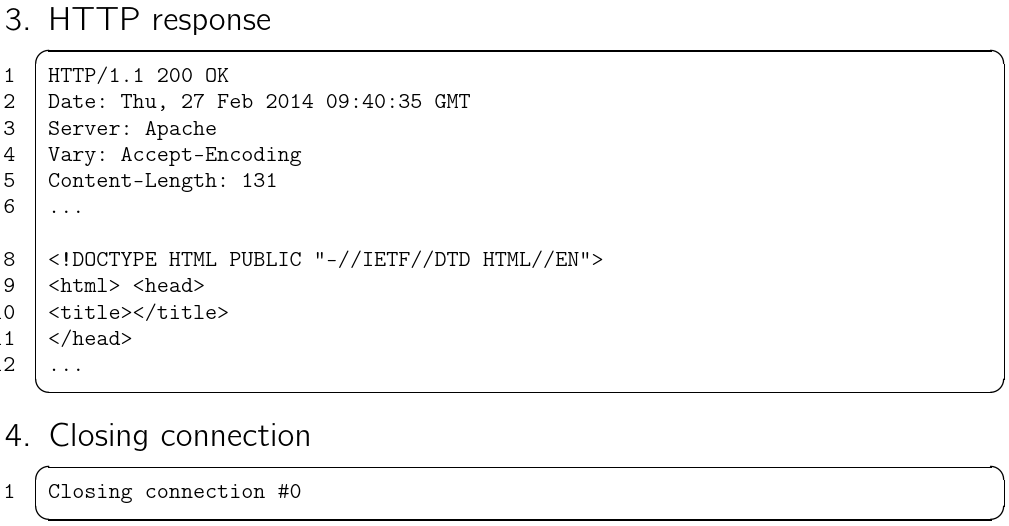
\includegraphics{fig/response.png}

\end{frame}

\begin{frame}{HTTP requests}

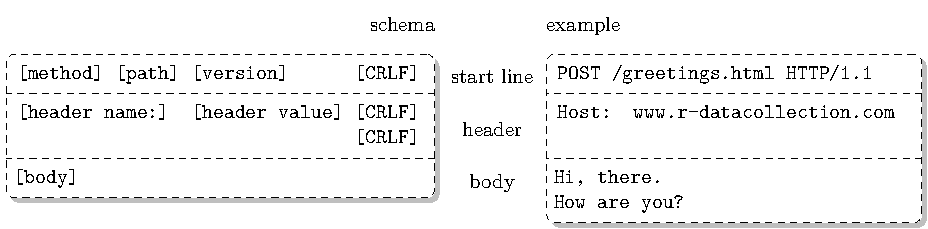
\includegraphics{fig/httprequest.pdf}

\end{frame}

\begin{frame}{HTTP responses}

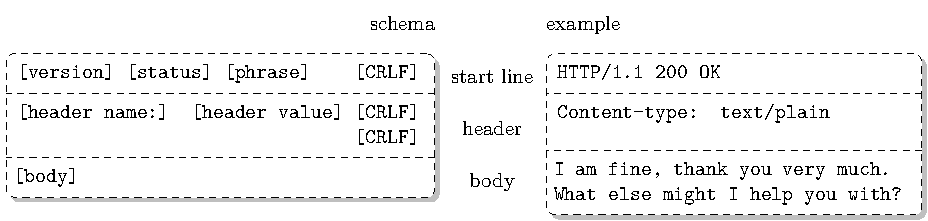
\includegraphics{fig/httpresponse.pdf}

\end{frame}

\begin{frame}{HTTP methods}

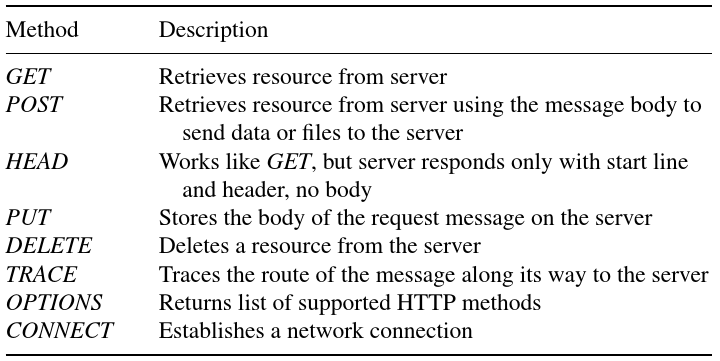
\includegraphics{fig/httpmethods.png}

\end{frame}

\begin{frame}{GET and POST}

\begin{itemize}
\tightlist
\item
  the same but GET puts all the information in the query string while
  POST puts the information in the body of the request
\end{itemize}

\end{frame}

\begin{frame}{Error codes}

\begin{itemize}
\tightlist
\item
  1xx : information
\item
  2xx : ok
\item
  3xx : redirect
\item
  4xx : client error
\item
  5xx : server error
\end{itemize}

\end{frame}

\begin{frame}[fragile]{Cookies}

\begin{enumerate}
\def\labelenumi{\arabic{enumi})}
\tightlist
\item
  client request to server
\item
  server response with header field ``Set-Cookie: sessionid=1234;
  path=/; domain=r-datacollection.com; expires=Mon, 31-Dec-2035 23:00:01
  GMT''
\item
  client request repeating the cookie values:
  \texttt{Cookie:\ sessionid=1234}
\end{enumerate}

\end{frame}

\begin{frame}{Identification}

\begin{itemize}
\tightlist
\item
  useragent (e.g.~R 3.2.3 / httr 1.0.0)
\item
  referer (Last\_Page\_I\_Visited.html)
\item
  from (e.g.~\href{mailto:bot@botnet.com}{\nolinkurl{bot@botnet.com}})
\item
  cookie (user=0112343asas)
\end{itemize}

\end{frame}

\begin{frame}{HTTPs}

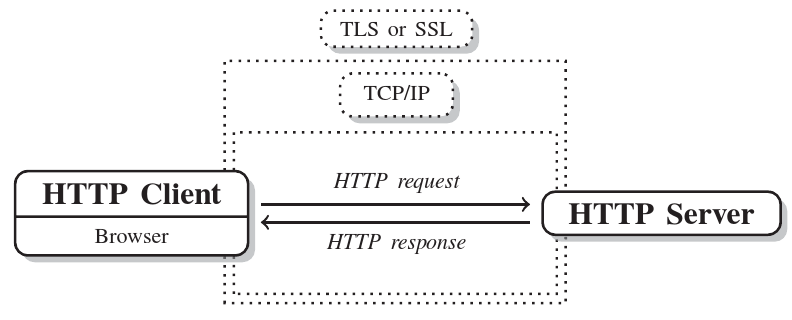
\includegraphics{fig/https.png}

\end{frame}

\begin{frame}{HTTP and httr}

\begin{itemize}
\tightlist
\item
  httr is a wrapper package to the curl package
\item
  httr functions mirror HTTP methods (GET, POST, PUT, DELETE, \ldots{})
\item
  httr tries to have very reasonable defaults (e.g.~handles cookies by
  default, follows redirections, \ldots{})
\item
  httr functions return the whole communication (request, response)
\end{itemize}

\end{frame}

\begin{frame}[fragile]{HTTP and httr - queries}

\begin{Shaded}
\begin{Highlighting}[]
\KeywordTok{library}\NormalTok{(httr)}
\KeywordTok{library}\NormalTok{(rvest)}
\end{Highlighting}
\end{Shaded}

\begin{verbatim}
## Loading required package: xml2
\end{verbatim}

\end{frame}

\begin{frame}[fragile]{HTTP and httr - queries}

\begin{Shaded}
\begin{Highlighting}[]
\NormalTok{url <-}\StringTok{ "http://www.r-datacollection.com/materials/http/GETexample.php"}

\KeywordTok{GET}\NormalTok{(url) %>%}\StringTok{ }\KeywordTok{content}\NormalTok{(}\DataTypeTok{as=}\StringTok{"text"}\NormalTok{) %>%}\StringTok{ }\KeywordTok{cat}\NormalTok{()}
\end{Highlighting}
\end{Shaded}

\begin{verbatim}
## No encoding supplied: defaulting to UTF-8.
\end{verbatim}

\begin{verbatim}
## Please specify your name!
## Please specify your age!
\end{verbatim}

\begin{Shaded}
\begin{Highlighting}[]
\KeywordTok{GET}\NormalTok{(url, }\DataTypeTok{query =} \KeywordTok{list}\NormalTok{(}\DataTypeTok{name=}\StringTok{"Joy"}\NormalTok{, }\DataTypeTok{age=}\StringTok{"22"}\NormalTok{))  %>%}\StringTok{ }
\StringTok{  }\KeywordTok{content}\NormalTok{(}\DataTypeTok{as=}\StringTok{"text"}\NormalTok{) %>%}\StringTok{ }\KeywordTok{cat}\NormalTok{()}
\end{Highlighting}
\end{Shaded}

\begin{verbatim}
## No encoding supplied: defaulting to UTF-8.
\end{verbatim}

\begin{verbatim}
## Hello Joy!
## You are 22 years old.
\end{verbatim}

\end{frame}

\begin{frame}[fragile]{HTTP and httr - useragent}

\begin{Shaded}
\begin{Highlighting}[]
\NormalTok{url <-}\StringTok{ "http://www.r-datacollection.com/materials/http/return.php"}

\KeywordTok{GET}\NormalTok{(url) %>%}\StringTok{ }\KeywordTok{content}\NormalTok{(}\DataTypeTok{as=}\StringTok{"text"}\NormalTok{) %>%}\StringTok{ }\KeywordTok{cat}\NormalTok{()}
\end{Highlighting}
\end{Shaded}

\begin{verbatim}
## No encoding supplied: defaulting to UTF-8.
\end{verbatim}

\begin{verbatim}
## GET /materials/http/return.php HTTP/1.1
## Connection: close
## Accept: application/json, text/xml, application/xml, */*
## Accept-Encoding: gzip, deflate
## Host: www.r-datacollection.com
## User-Agent: libcurl/7.35.0 r-curl/0.9.6 httr/1.1.0
## Authorization: 
## 
\end{verbatim}

\end{frame}

\begin{frame}[fragile]{HTTP and httr - useragent}

\begin{Shaded}
\begin{Highlighting}[]
\KeywordTok{GET}\NormalTok{(url, }\KeywordTok{user_agent}\NormalTok{(}\StringTok{"httr"}\NormalTok{)) %>%}\StringTok{ }\KeywordTok{content}\NormalTok{(}\DataTypeTok{as=}\StringTok{"text"}\NormalTok{) %>%}\StringTok{ }\KeywordTok{cat}\NormalTok{()}
\end{Highlighting}
\end{Shaded}

\begin{verbatim}
## No encoding supplied: defaulting to UTF-8.
\end{verbatim}

\begin{verbatim}
## GET /materials/http/return.php HTTP/1.1
## Connection: close
## Accept: application/json, text/xml, application/xml, */*
## Accept-Encoding: gzip, deflate
## Host: www.r-datacollection.com
## User-Agent: httr
## Authorization: 
## 
\end{verbatim}

\end{frame}

\begin{frame}[fragile]{HTTP and httr - auto parsing}

\begin{Shaded}
\begin{Highlighting}[]
\NormalTok{url <-}\StringTok{ "http://www.r-datacollection.com/materials/html/OurFirstHTML.html"}

\KeywordTok{GET}\NormalTok{(url)  %>%}\StringTok{ }\KeywordTok{content}\NormalTok{() %>%}\StringTok{ }
\StringTok{  }\KeywordTok{html_nodes}\NormalTok{(}\StringTok{"title"}\NormalTok{) %>%}\StringTok{ }
\StringTok{  }\KeywordTok{html_text}\NormalTok{()}
\end{Highlighting}
\end{Shaded}

\begin{verbatim}
## No encoding supplied: defaulting to UTF-8.
\end{verbatim}

\begin{verbatim}
## [1] "First HTML"
\end{verbatim}

\begin{Shaded}
\begin{Highlighting}[]
\KeywordTok{GET}\NormalTok{(url)  %>%}\StringTok{ }\KeywordTok{content}\NormalTok{(}\DataTypeTok{as=}\StringTok{"text"}\NormalTok{)}
\end{Highlighting}
\end{Shaded}

\begin{verbatim}
## No encoding supplied: defaulting to UTF-8.
\end{verbatim}

\begin{verbatim}
## [1] "<!DOCTYPE html>\n <html>\n   <head>\n     <title>First HTML</title>         \n   </head>\n   <body>\n     I am your first HTML-file!\n   </body>\n </html>\n"
\end{verbatim}

\end{frame}

\begin{frame}[fragile]{HTTP and httr - follow location}

\begin{Shaded}
\begin{Highlighting}[]
\NormalTok{url <-}\StringTok{ "http://www.r-datacollection.com/materials/http/redirect.php"}
\KeywordTok{try}\NormalTok{(}\KeywordTok{readLines}\NormalTok{(url))}

\KeywordTok{GET}\NormalTok{(url)  %>%}\StringTok{ }\KeywordTok{content}\NormalTok{(}\DataTypeTok{as=}\StringTok{"text"}\NormalTok{)}
\end{Highlighting}
\end{Shaded}

\begin{verbatim}
## No encoding supplied: defaulting to UTF-8.
\end{verbatim}

\begin{verbatim}
## [1] "<html>\r\n <head>\r\n  <title>redirected</title>\r\n </head>\r\n <body>\r\n You were redirected - I think. <br><br>\r\n \r\n If not, try this: <a href=\"redirect.php\">redirect.php</a>\r\n </body>\r\n</html>"
\end{verbatim}

\end{frame}

\begin{frame}[fragile]{HTTP and httr - (auto) cookies}

\begin{Shaded}
\begin{Highlighting}[]
\NormalTok{url <-}\StringTok{ "http://www.r-datacollection.com/materials/http/Cookies.php"}

\KeywordTok{content}\NormalTok{(}\KeywordTok{GET}\NormalTok{(url))}
\end{Highlighting}
\end{Shaded}

\begin{verbatim}
## No encoding supplied: defaulting to UTF-8.
\end{verbatim}

\begin{verbatim}
## {xml_document}
## <html>
## [1] <body>\n  <p>Hallo, who are you?</p>\n</body>
\end{verbatim}

\begin{Shaded}
\begin{Highlighting}[]
\KeywordTok{content}\NormalTok{(}\KeywordTok{GET}\NormalTok{(url))}
\end{Highlighting}
\end{Shaded}

\begin{verbatim}
## No encoding supplied: defaulting to UTF-8.
\end{verbatim}

\begin{verbatim}
## {xml_document}
## <html>
## [1] <body>\n  <p>Ah, nice to meet you again. </p>\n</body>
\end{verbatim}

\end{frame}

\begin{frame}[fragile]{HTTP and httr - methods}

\begin{Shaded}
\begin{Highlighting}[]
\NormalTok{url <-}\StringTok{ "http://www.r-datacollection.com/materials/http/returnquery.php"}

\KeywordTok{GET}\NormalTok{(url, }\DataTypeTok{query=}\KeywordTok{list}\NormalTok{(}\DataTypeTok{a=}\DecValTok{1}\NormalTok{,}\DataTypeTok{b=}\DecValTok{3}\NormalTok{)) %>%}\StringTok{ }\KeywordTok{content}\NormalTok{(}\DataTypeTok{as=}\StringTok{"text"}\NormalTok{) %>%}\StringTok{ }\KeywordTok{cat}\NormalTok{()}
\end{Highlighting}
\end{Shaded}

\begin{verbatim}
## No encoding supplied: defaulting to UTF-8.
\end{verbatim}

\begin{verbatim}
## <pre>
## parameters submitted via GET: (name) : (value)
## a  : 1
## b  : 3
## 
## 
## parameters submitted via POST: (name) : (value)
## 
## </pre>
\end{verbatim}

\end{frame}

\begin{frame}[fragile]{HTTP and httr - methods}

\begin{Shaded}
\begin{Highlighting}[]
\NormalTok{url <-}\StringTok{ "http://www.r-datacollection.com/materials/http/returnquery.php"}

\KeywordTok{POST}\NormalTok{(url, }\DataTypeTok{body =} \KeywordTok{list}\NormalTok{(}\DataTypeTok{a=}\DecValTok{1}\NormalTok{,}\DataTypeTok{b=}\DecValTok{3}\NormalTok{)) %>%}\StringTok{ }\KeywordTok{content}\NormalTok{(}\DataTypeTok{as=}\StringTok{"text"}\NormalTok{) %>%}\StringTok{ }\KeywordTok{cat}\NormalTok{()}
\end{Highlighting}
\end{Shaded}

\begin{verbatim}
## No encoding supplied: defaulting to UTF-8.
\end{verbatim}

\begin{verbatim}
## <pre>
## parameters submitted via GET: (name) : (value)
## 
## 
## parameters submitted via POST: (name) : (value)
## a  : 1
## b  : 3
## 
## </pre>
\end{verbatim}

\end{frame}

\begin{frame}[fragile]{HTTP and httr - headers}

\begin{Shaded}
\begin{Highlighting}[]
\NormalTok{url <-}\StringTok{ "http://www.r-datacollection.com/materials/http/return.php"}

\KeywordTok{GET}\NormalTok{(url, }\KeywordTok{add_headers}\NormalTok{(}\DataTypeTok{from=}\StringTok{"bot@botnet.de"}\NormalTok{, }\DataTypeTok{referrer=}\StringTok{"botnet.de"}\NormalTok{)) %>%}\StringTok{ }
\StringTok{  }\KeywordTok{content}\NormalTok{(}\DataTypeTok{as=}\StringTok{"text"}\NormalTok{) %>%}\StringTok{ }\KeywordTok{cat}\NormalTok{()}
\end{Highlighting}
\end{Shaded}

\begin{verbatim}
## No encoding supplied: defaulting to UTF-8.
\end{verbatim}

\begin{verbatim}
## GET /materials/http/return.php HTTP/1.1
## Connection: close
## Referrer: botnet.de
## From: bot@botnet.de
## Accept: application/json, text/xml, application/xml, */*
## Cookie: id=d10b3aaa226397acafc2275ba02a2586
## Accept-Encoding: gzip, deflate
## Host: www.r-datacollection.com
## User-Agent: libcurl/7.35.0 r-curl/0.9.6 httr/1.1.0
## Authorization: 
## 
\end{verbatim}

\end{frame}

\end{document}
